\documentclass[11pt,fleqn,a4paper,halfparskip]{article}
\usepackage[ngerman]{babel}
\usepackage[utf8]{inputenc}
\usepackage{textcomp}
\usepackage{graphicx}
\usepackage{upgreek}
\usepackage{floatflt}
\usepackage{amsmath}
\usepackage{amssymb}
\usepackage[final]{pdfpages}
\usepackage[a4paper, left=2cm, right=2cm, top=2cm]{geometry}
\usepackage[T1]{fontenc}
\usepackage{lmodern}
\renewcommand*\familydefault{\sfdefault}

\setcounter{section}{-1}

\title{Grundbau Beleg}
\author{Paul Debus \and Matrikelnummer: 110113}

\begin{document}
\pagenumbering{roman}
\maketitle
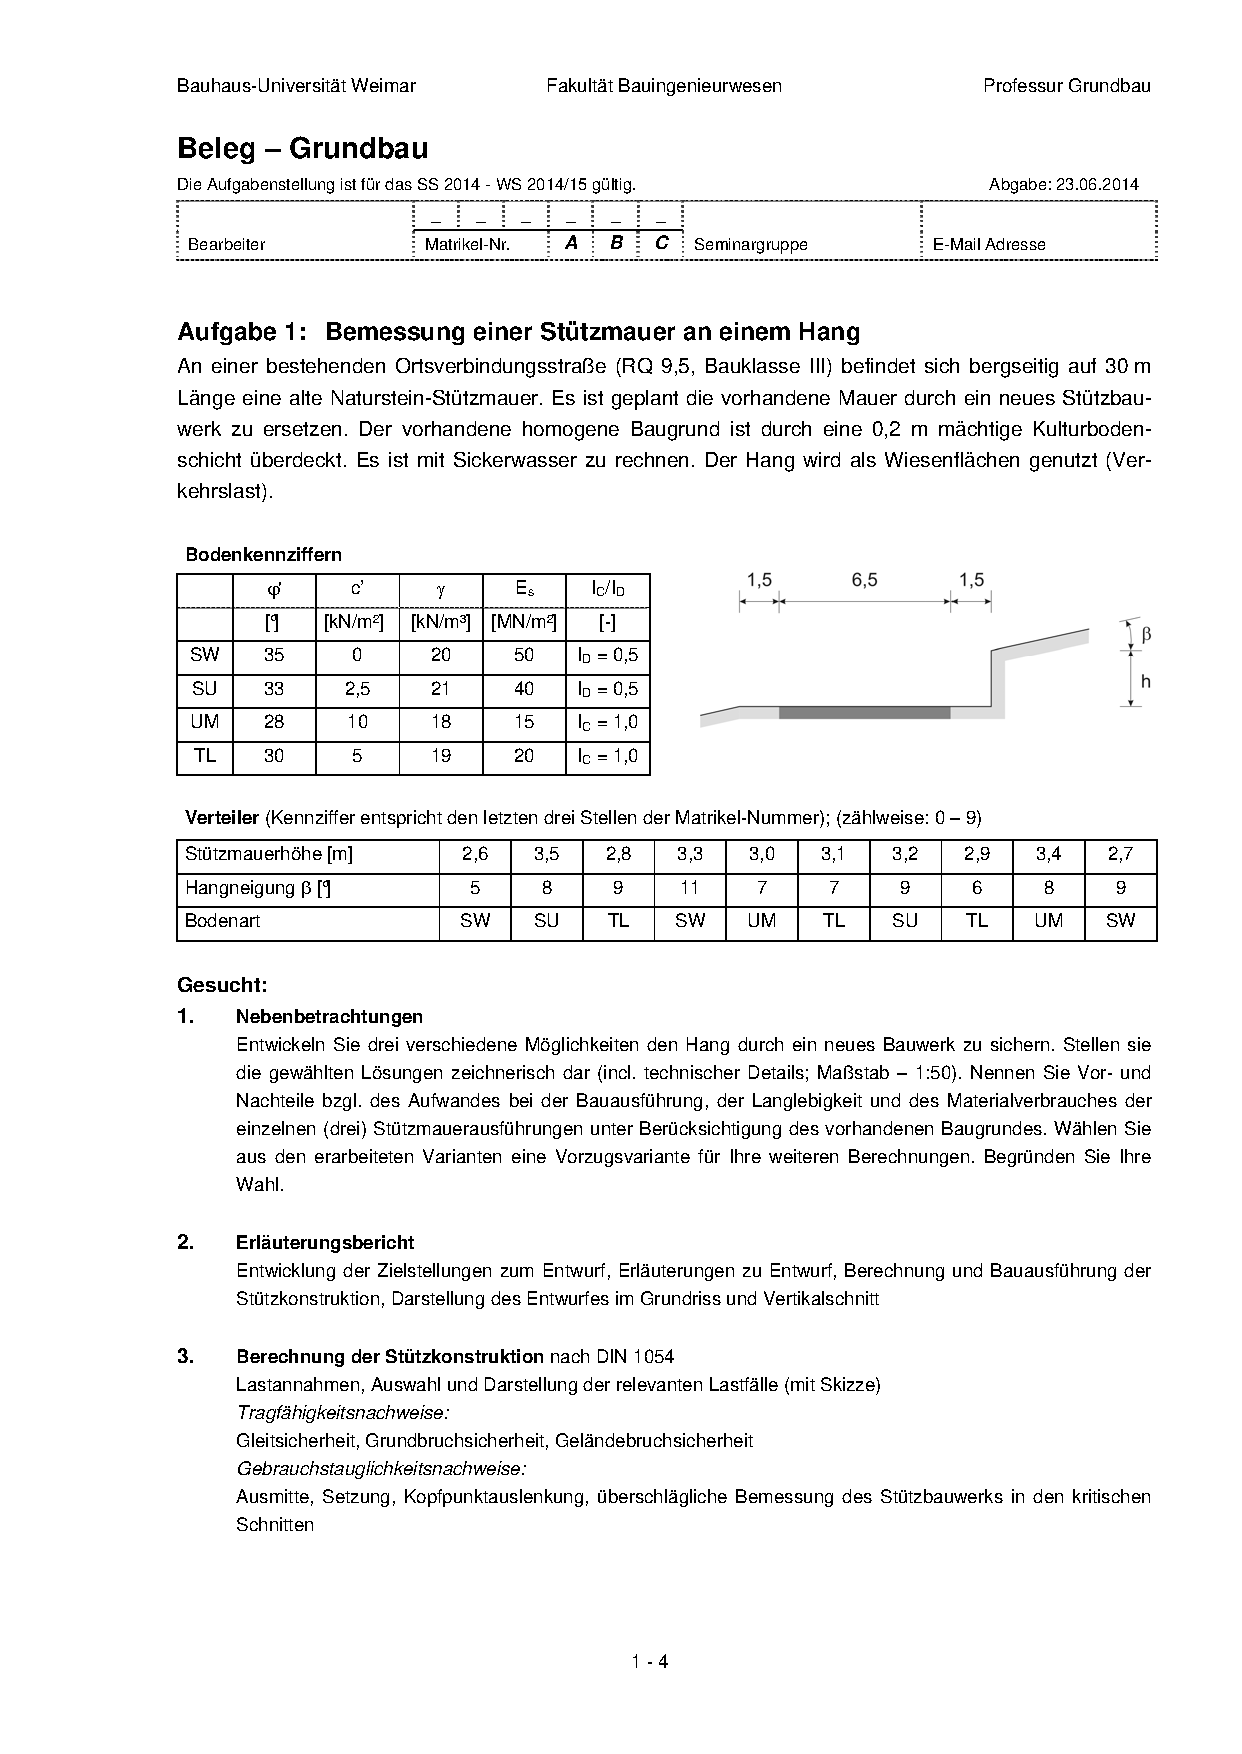
\includepdf[pages=1,pagecommand=\section{Aufgabenstellung}, scale=0.9]{aufgabe.pdf}
\includepdf[pages=2-,pagecommand={},scale=0.9]{aufgabe.pdf}
\tableofcontents
\newpage
\pagenumbering{arabic}
\section{Aufgabe 1}
\subsubsection*{Festlegung der eigenen Parameter aus Verteiler}
Matrikelnummer 110113
\begin{itemize}
\item Stützmauerhöhe 3,3m
\item Hangneigung $11^\circ$
\item Bodenart SW
\item $\varphi $' = $35^\circ$
\item c' = 0 [kN/m²]
\item $\gamma$ = 20 [kN/m³]
\item $E_s$ = 50 [MN/m²]
\item $l_c/l_o$ = 0.5
\end{itemize}
\subsection{Erläuterungsbericht}
\subsubsection*{Charakteristik der Aufgabe und des Standortes}
Es soll eine 30m lange Stützmauer entlang einer Straße erneuert werden. Dazu soll die vorhandene Natursteinmauer durch ein neues Bauwerk ersetzt werden. Der anstehende Boden ist ein abgestufter Kies, der von 0.2m Mutterboden bedeckt wird. Der Hang wird als Wiese genutzt und es mit Sickerwasser zu rechnen. \\
Im folgenden werden drei Varianten für das neue Bauwerkt beschrieben, von denen dann eine ausgewählt und bemessen wird.
\subsubsection*{Variante 1: Spundwand} 
Eine Spundwand ist ein in den Boden gerammtes Stahlprofil, welches als wie ein Kragträger wirkt. Durch den guten Verbund der einzelnen Elemente, sind Spundwände praktisch wasserdicht. Ab einer gewissen Höhe verankert man Spundwände horizontal in den Boden um Verformungen und Momente in der Baugrubensohle zu reduzieren und damit die Einbindelänge. Spundwände werden vor allem für den Baugrubenverbau eingesetzt, da sie sehr schnell zu montieren sind und nach dem Abbau wieder verwendet werden können. Für dauerhafte Bauten werden Spundwände besonders im Hafenbau eingesetzt, aber auch im Straßenbau zur Hangsicherung. \\
Der Aufwand bei der Bauausführung ist sehr gering, da die Spundwand einfach hinter der schon bestehenden Wand eingerammt werden kann und man diese danach abtragen kann. Bei anderen Befestigungen wie z.B. einer Winkelmauer ist eine Baugrube erforderlich, die allein schon eine Spundwand zur Absicherung braucht. Der Montageaufwand ist daher im Vergleich zu anderen Verfahren sehr gering. \\
Da Spundwände aus Stahl hergestellt werden, muss sich auch um Korrosionsschutz Gedanken gemacht werden. Gerade auf der Seite des anstehenden Bodens ist dieser nur sehr schwer zu leisten, sodass eine Spundwand nicht verlässlich vor Korrosion geschützt werden kann. Da ein Dauerbauwerk auf mehrere Jahrzehnte ausgelegt wird (wenn nicht sogar noch länger), wird es irgendwann zu Einschränkungen der Tragfähigkeit einer Spundwand kommen. \\
Für kurzzeitige Verbaue sind Spundwände sehr gut geeignet, bei Dauerbauwerken kann man Probleme mit der Haltbarkeit bekommen.
\newpage
\begin{figure}[h]
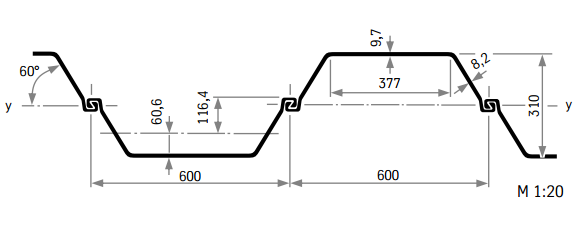
\includegraphics[scale=0.5]{Spundwandschnitt.png}
\caption{Schnitt durch ein Spundwandprofil Larsen 603 \cite[2.1.1 S.10]{spund}}
\end{figure}
\begin{figure}[h!]
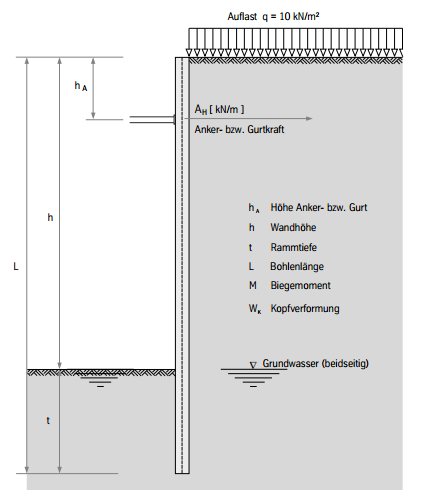
\includegraphics[scale=0.4]{Spundwandlangs.png}
\caption{Längsschnitt durch eine Spundwand \cite[1.6 S.10]{spund}}
\end{figure}
\newpage
\subsubsection*{Variante 2: Gabione}
Gabionen sind mit Steinen gefüllte Drahtkörbe, die zu einer Mauer aufgebaut werden und wie eine Gewichtsmauer wirken. Bei der Füllung ist auf die Auswahl von frost- und Witterungsbeständigem Material zu achten. Die Füllung kann geschüttet werden (wirtschaftlich) oder per Hand gestapelt werden (ästhetisch). Gabionen werden in der Landschaftsarchitektur, im Wasserbau sowie im Straßen- und Wegebau zum Aufbau von Wällen, zur Errichtung von Sicht- oder Lärmschutzanlagen, zur Böschungsbefestigung und als Stützmauer (etwa als Alternative zu konventionellen Trockenmauern in Weinbergen) eingesetzt. \\
Ein Vorteil der Gabionen gegenüber z.B. einer Spundwand ist die gute Anpassungsfähigkeit dem Gelände gegenüber. Außerdem sind sie durch geringen technologischen Aufwand und günstige Baustoffe relativ wirtschaftlich herzustellen. Außerdem sind sie ökologisch nachhaltiger als andere Befestigungen, da sie sich leicht begrünen lassen und so Kleintieren einen Lebensraum bieten können. \\
Früher wurden Gabionen so geplant, dass sie von der Vegetation durchwachsen werden, während gleichzeitig der Draht der Körbe verrostet, sodass wie eine natürliche Befestigung wirkt. Heute werden die Körbe aus verzinktem Stahl gefehrtigt, sodass sie auch mehrere Jahrzente stabil bleiben. Bei grober Fülung der Körbe sind Gabionenwände auch wasserdurchlässig und erhalten so den natürlichen Wasserfluss.\\
Die Herstellung der Gabionenwand ist nicht aufwändig und geht relativ schnell, je nach Qualität des vorhandenen Fundamentes der bisherigen Mauer, sind Betonarbeiten nötig, die den Umfang der Projektes vergrößern.
\begin{figure}[h!]
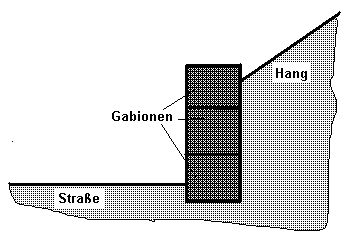
\includegraphics[scale=0.8]{Gabionenwand.png}
\caption{Längsschnitt durch eine Gabionenwand \cite{gabio}}
\end{figure}
\begin{figure}[h!]
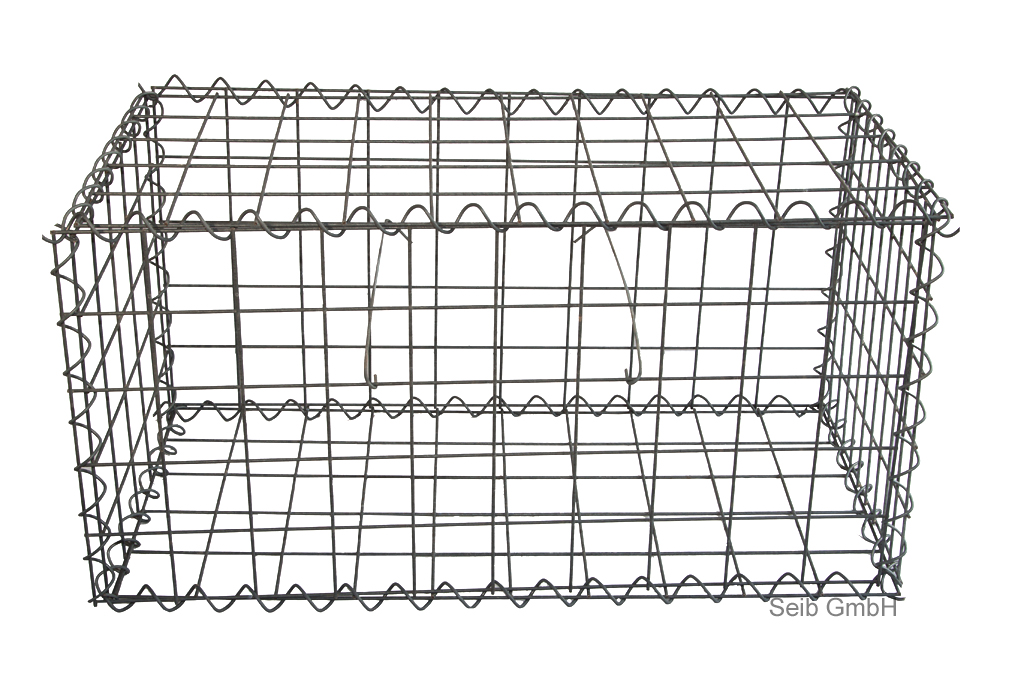
\includegraphics[scale=0.2]{gabione.jpg}
\caption{Ein Gabionenkorb \cite{gabio2}}
\end{figure}
\newpage
\subsubsection*{Variante 3: Gewichtsmauer}
Gewichtsmauern sind massive, meist aus unbewehrtem Beton hergestellte Hangsicherungsbauwerke. Sie gleichen in Bau- und Wirkungsweise den Gewichtsstaumauern aus dem Wasserbau. \\
Gewichtsmauern lassen sich sehr gut an das Gelände anpassen und können auch gut in großen Maßen hergestellt werden. Allerdings brauchen sie relativ viel Material und haben einen relativ langen Herstellungsprozess. Außerdem muss eine Baugrube ausgehoben werden. \\
In der Pflege im Bestand des Bauwerkes sind Betonmauern generell sehr einfach, da Beton ein wetterfestes Material ist.
\begin{figure}[h!]
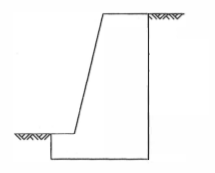
\includegraphics[scale=0.8]{gewichtsmauer.png}
\caption{Längsschnitt durch eine Gewichtsmauer \cite[11.63]{gewichtsmauer}}
\end{figure}
\subsubsection*{Auswahl einer der Varianten}
Jede der drei vorgestellten Varianten hat besondere Vorzüge und ist für bestimmte Szenarien besser geeignet als die anderen. In diesem Fall wähle ich die \textbf{Gabione}. Diese Wahl treffe ich besonders aufgrund des Sickerwassers, das an diesem Hang eintrifft. Bei anderen, wasserundurchlässigen Bauwerken muss sich um die Wasserhaltung gesondert Gedanken gemacht werden und es müssen zusätzliche Entwässerungsanlagen geplant werden. Dies alles ist bei Gabionen nicht der Fall. Weitere Gründe für die Gabione sind eine Tragweise vergleichbar mit der einer Gewichtsmauer, verbunden mit einer Montagegeschwindigkeit, die eher einer Spundwand entspricht. Außerdem kann man dieses Bauwerk sehr gut an die Form des Hanges anpassen. \\
In diesem Fall kommt noch dazu, dass sowohl das Material der vorhandenen Stützmauer als auch der anstehende Boden verwendet werden kann, die Körbe zu befüllen. \\
In meiner Erfahrung sind Gabionen sehr häufig anzutreffende Bauwerke für diesen Zweck. Auch optisch passt eine Gabione besser in die Landschaft einer Wiese, als eine doch sehr massive Stahl- oder Betonkonstruktion.
\subsubsection*{Konstruktiv-technologische Festlegungen}
Aus technologischen Gründen werden Körbe von 1m Höhe, 2m Tiefe und 3m Breite verbaut. Um die nötige Höhe von 3.3m zu überwinden, werden 4 Körbe übereinander gestapelt. Daraus ergibt sich eine Einbindetiefe der Körbe von 70cm. Die Körbe werden wie eine Treppe mit jeweils 30cm Versatz aufeinander gestapelt. Insegesamt ergibt das einen Versatz von 90cm, also einen Wandneigungswinkel von -12.7$^\circ$.\\
Um eine monolithische Wirkung 
Da die Körbe erst vor Ort auf der Baustelle gefüllt werden, wir das vorhandene Material verwendet. Außerdem kann das abgetragene Material der alten Mauer verwendet werden. Allerdings wird die Wichte etwas reduziert angesetzt, da die feinen Anteile aus den Körben heraus rieseln. Ich setze eine Wichte von $16kN/m^3$ an. 
\newpage
\subsubsection*{Bauablauf}
\begin{itemize}
\item Absperrung der Straße
\item Abtragen des Mutterbodens oberhalb
\item Einrammen einer Spundwand als Baugrubensicherung
\item Rückbau der vorhandenen Wand und Abtragen des anstehenden Bodens
\item Ausheben der Baugrube 
\item Aufstellen der Gabionen und lagenweises Hinterfüllen und verdichten des Bodens
\item Nach jeder neuen Lage die Blöcke mit der Lage darunter monolithisch verbinden
\item Bau eines Entwässerungsgrabens entlang der Straße am Fuße der Stützmauer
\item Entfernen der Spundwand und der Absperrung
\item Wiederherstellung der Wiese
\end{itemize}
\subsection{Bemessung}
\subsubsection{Lastannahmen und Lastfälle}
Die einwirkenden Kräfte aus dem Boden ergeben sich aus der Aufgabenstellung. Dazu wird auf der Wiese eine Last von $20kn/m^2$ angesetzt, davon $10kN/m^2$ als ständige Last und $10kN/m^2$ als Verkehrslast.
\subsubsection*{Lastfall aktiver Erddruck und ständige Auflast}
Annahme: $\delta_a = |\alpha| = 12.7^\circ \rightarrow E_{av} = 0 $ \cite[S.149]{wsp} \\
\begin{equation*}
E_a = E_{ah} =  1/2 \gamma ' h^2 K_{ag} + p h K_{ap} - c h K_{ac}
\end{equation*}
Der Boden hat keine Kohäsion. Deshalb:
\begin{equation*}
E_a = E_{ah} =  1/2 \gamma ' h^2 K_{ag} + p h K_{ap}
\end{equation*}
\begin{equation*}
K_{agh} = \left[\frac{\cos(\varphi - \alpha)}{\cos \alpha \left(1+ \sqrt{\frac{\sin(\varphi + \delta_a)*\sin(\varphi - \beta)}{\cos(\alpha - \beta) * \cos(\alpha + \delta_a)}}\right)}\right]^2
=
\left[\frac{\cos(35^\circ - (-12.7^\circ))}{\cos (-12.7^\circ) \left(1+ \sqrt{\frac{\sin(35^\circ + 12.7^\circ)*\sin(35^\circ - 11^\circ)}{\cos((-12.7^\circ) - 11^\circ) * \cos((-12.7^\circ) + 12.7^\circ)}}\right)}\right]^2 
\end{equation*}
\begin{equation*}
K_{agh} = 0.0.1925
\end{equation*}
\begin{equation*}
K_{aph} = K_{agh}\frac{\cos\alpha \cos\beta}{\cos(\alpha - \beta)} = 0.2013
\end{equation*}
\begin{equation*}
E_a = E_{ah} =  1/2 \gamma ' h^2 K_{ag} + p h K_{ap} = 27.6kN/m
\end{equation*}
\begin{equation*}
y_{E_a} = \frac{2e_{ah1} + e_{ah2}}{e_{ah1} + e_{ah2}} \frac{h}{3} = 1.512m
\end{equation*}
\newpage 
\begin{figure}
\vspace{10cm}
\caption[Erddruckverteilung Aufgabe 1]{Erddruckverteilung \cite{me}}
\end{figure}
\subsubsection*{Lastfall Verkehrslast}

\subsubsection{Ermittlung der Einwirkungen}
\begin{equation*}
G_k = Tiefe_{Block} * Höhe_{Block} * Anzahl_{Blöcke} * \gamma_{Block} = 2m * 1m * 4 * 16kN/m^3 = 128kN/m
\end{equation*}
$\hspace{1cm} V_k = 0 $ Aus Annahme für aktiven Erddruck \\
$\hspace{1cm} H_k = 27.6kN/m $ Aktiver Erddruck \\
Schnittgrößen in der Sohlfuge: \\
$\hspace{1cm} N_k = V_k + G_k = 128Kn/m $\\
$\hspace{1cm} T_k = H_k = 27.6kN/m $ \\
$\hspace{1cm} M_k = H_k * y_{E_a} = 27.6kN/m * 1.512m = 41.719kNm/m $ \\
\begin{equation*}
e = \frac{M_k}{N_k} = \frac{41.719kNm/m}{120kN/m} = 0.326m
\end{equation*}
\subsubsection{Nachweis Kippsicherheit GZ EQU}
Berechnungen nach \cite[S.97]{wsp}. Das Verfahren ist anwendbar, da mindestens mitteldicht gelagerter nichtbindiger Boden vorliegt.\\ 
Prüfen, ob die Sohldruckresultierende aus ständigen Belastungen innerhalb der ersten Kernweite liegt: \\
Bedingung: $ e \le b/6 =0.33m$ \\
$ 0.326m \le 0.33m \checkmark$ \\
\newpage
Prüfen, ob die Sohldruckresultierende aus ständigen und veränderlichen Belastungen innerhalb der zweiten Kernweite liegt:\\
Bedingung: $e \le b/3 = 0.66m$\\
Rechnung analog zu nur ständige Einwirkungen.\\
$E_{a,2} = 34.24kN/m$ \\
$M_{k,2} = 44.98kNm/m$ \\
$e_2 = 0.351m \le 0.66m \checkmark$
\subsubsection{Nachweis Grundbruchsicherheit GZ GEO.2}
Berechnung nach \cite[S.99]{wsp}. \\
\textbf{Beanspruchungen:}\\
$V_d = V_G*\gamma_G = 128kN/m * 1.35 = 172.8kN/m$ \\
\\
\textbf{Widerstände}\\
Berechnung der geometrischen Parameter: \\
$ a' = 1m$ Meterstreifen, da Streifenfundament \\
$ b' = b - 2e = 2m - 2*0.326m = 1.348m$ \\
$ \tan\delta = T/N = 0.216 $ \\
$ \delta = 12.55^\circ \rightarrow$ Der Gleitkörper verschiebt sich in Richtung von T. 
\\
Bestimmung des Widerstandes (keine Kohäsion): \\
$R_n = a'b' (\gamma_1 d N_d + \gamma_2 b' N_b)$\\
\\
\begin{tabular}{|l|r|r|}
\hline
 & \multicolumn{1}{l|}{\textbf{Gründungstiefe}} & \multicolumn{1}{l|}{\textbf{Gründungsbreite}} \\ \hline
\textbf{Tragfähigkeit} & 33.296 & 22.614 \\ \hline
\textbf{Form} & 1 & 1 \\ \hline
\textbf{Lastneigung} & 0.615 & 0.483 \\ \hline
\end{tabular}\\
\\
$ N_d = N_{d,0} \upnu_d i_d = 33.296 * 1 * 0.615 = 20.485$ \\
$ N_b = N_{b,0} \upnu_b i_b = 22.614 * 1 * 0.483 = 10.913$ \\
$ R_n = 1 * 1.348 * (20 * 0.7 * 20.485 + 20 * 1.348 * 10.913) = 783.913kN/m$\\
$R_d = R_n/\gamma_{R,v} = 783.913  / 1.4 = 559.938kN/m$ \\
\\
$N_d = 172.8kN/m < R_d = 559.938kN/m$ $\checkmark$ \\
Grundbruchsicherheitsnachweis erfüllt!
\subsubsection{Nachweis Gleitsicherheit GZ GEO-2}
Berechnung nach \cite[S.98]{wsp}. Der Erdwiderstand auf der anderen Seite wird nicht angesetzt.\\
\textbf{Beanspruchungen:}\\
$H_d = H_{G,k}\gamma_G + H_{Q,k}\gamma_Q$ \\
$H_{G,k} = E_{agh} = 27.6kN/m $\\
$H_{Q,k} = E_{aph} = phK_{ap} = 10kN/m^2*3.3m*0.2013 = 6.643kN/m $\\
$H_d = 27.6kN/m * 1.35 + 6.643kN/m * 1.5 = 47.2245kN/m$\\
\newpage
\textbf{Widerstände:}\\
$R_d = R_k/\gamma_{R,h} = R_k/1.1$ \\
$R_k = V'_k \tan\delta_k$\\
$V'_k = G_k + E_{a,v} = G_k + 0 = 128kN/m$\\
$\delta_k = \varphi$ (max $35^\circ$) = $35^\circ$\\
$R_k = 128kN/m * \tan(35^\circ) = 89.63kN/m$ \\
$R_d = R_k/1.1 = 89.63kN/m/1.1 = 81.48kN/m$ \\
\\
$H_d = 47.2245kN/m < R_d = 81.48kN/m \checkmark$ \\
Gleitsicherheitsnachweis erfüllt!

\subsubsection{Nachweis der Setzungen}
Berechnung nach \cite[S.68]{wsp}. Bei einem Streifenfundament keine Verdrehung in der langen Richtung, da keine Ausmitte der Last. \\
Annahme: a = 10b und z = 2b\\
Gesamtsetzung: $ s = s_m \pm s_x$ \\
Setzungsbeiwerte und Verkantungsbeiwerte:\\
Auslesen aus Tabelle \cite[s.69]{wsp} für f(10;2):\\
\begin{itemize}
\item $f = 0.9655$
\item $f_x = 0.0108$
\item $f_y = 0.4482$ nicht benötigt
\end{itemize}
Mittlere Setzung aus zentrischer Last:
\begin{equation*}
s_m = \frac{\sigma_1b}{E_m}f
\end{equation*}
$\hspace{1cm} E_m = E_s/\kappa = \frac{50}{2/3} = 75MN/m^2$, $\kappa = 2/3$ für Sand und Schluff
\begin{equation*}
\sigma_1 = \frac{V}{ab} = \frac{128}{2*20} = 3.2kN/m^2
\end{equation*}
$\hspace{1cm} s_m = \frac{3.2kN/m^2*2m}{75000kN/m^2}0.9655 = 0.000082m = 0.082mm $ \\
\\
Verdrehung durch ausmittige Last:\\
\begin{equation*}
s_x = \tan\alpha_y * \frac{a}{2}
\end{equation*}
\begin{equation*}
\tan\alpha_y = \frac{M_y}{b^3E_m}f_x
\end{equation*}
$\hspace{1cm} M_y = -Ve_x = 128kN/m * 0.326m = -41.73kNm/m $
\begin{equation*}
\tan\alpha_y = \frac{-41.73kNm/m}{(2m)^3*75000kN/m^2} 0.0108 = -7.5114*10^{-7}m
\end{equation*}
$\hspace{1cm} s_x = \tan\alpha_y * a/2 = -7.5114*10^{-7} * 20 / 2 = -7.5114*10^{-6}m = -0.0075114mm $
\\
\textbf{Gesamtsetzung:}\\
Die Gesamtsetzungen sind weit weniger als 1mm, also sehr gering und damit nicht relevant.



\subsection{Konstruktionszeichnungen}
\subsection{Nebenbetrachtungen}


\newpage
\section{Aufgabe 2}
\subsubsection*{Festlegung der eigenen Parameter aus Verteiler}
Matrikelnummer: 110113\\
\begin{itemize}
\item Baugrubentiefe: 4.9m
\item Bodenart: SW
\item $\varphi': 32^\circ$
\item c' = 0
\item $\gamma = 18kN/m^3$
\item $E_s = 60MN/m^2$
\item $l_D = 0.5$
\end{itemize}
\subsection{Entwurf der Verbaukonstruktion}
\subsubsection{Erläuterungsbericht}
Die zu stützende Baugrube hat eine Tiefe von 4.9m. Das gewählte Bauwerk ist eine einfach ausgesteifte und frei aufgelagerte Trägerbohlwand. Der Anker wird nach 1m Höhe, also 3.9m über der Baugrubensohle angebracht. Er soll helfen die Lasten aus der benachbarten Bebauung aufzunehmen und gleichzeitig die Verformungen so gering zu halten, dass das benachbarte Wohnhaus nicht beschädigt wird. \\
Bei der Baudurchführung werden zuerst die Träger in den Boden gerammt. Dann wird begonnen die Baugrube auszuheben. Dabei werden nach und nach die Bohlen eingebracht und mit Holzkeilen befestigt. Nach etwa 1.5m bis 2m wird der Aushub pausiert um die Anker einzubringen. Diese Aushubtiefe ist absolut unproblematisch, da die Träger auf eine größere Grube bemessen werden. Nach dem Einbringen der Träger, wird die Grube zu Ende ausgehoben und der Neubau kann beginnen. Nach Abschluss der Bauarbeiten erfolgt der Rückbau genau in umgekehrter Reihenfolge zum Einbau.\\
Es ist zu beachten, dass bauzeitlich mit Grundwasser in der Baugrubensohle gerechnet werden muss.

\subsubsection{Vertikalschnitt und Grundriss}
\subsubsection{Geometrische Definition und Festlegung der zu ermittelnden Größen}
Für die Ausführung wichtige Größen sind:\\
 Einbindetiefe der Träger, Trägerabstände, Profil der Träger, Bohlenlänge, Profil der Bohlen, Ankerabstand, Ankermaße. \\
\\
Annahmen die vor der Bemessung getroffen werden: \\
- Trägerabstand 2m\\
- Ankerhöhe 1m unter Geländeoberkante\\
- Boden genügend tragfähig um für Bohleneinbau ausheben zu können.
\newpage
\subsection{Bemessung}
Berechnung nach \cite[S.137ff]{wsp}
\subsubsection{Lastannahmen}
\textbf{Ständige Einwirkungen}
\begin{itemize}
\item Eigenlasten der Baugrubenkonstruktion
\item Erddruck infolge Bodeneigengewicht
\item Erddruck infolge ständiger Eigenlast benachbarter Bauwerke
\item Erddruck infolge einer veränderlichen großflächigen Gleichlast von $10kN/m^2$, die als ständige Gleichlast betrachtet wird
\item Wasserdruck aus Grundwasser in der Baugrubensohle
\end{itemize}
\textbf{Veränderliche Einwirkungen}
\begin{itemize}
\item Erddruck infolge Verkehrslasten benachbarter Bauwerke
\end{itemize}
\subsubsection{Lastfälle}
\textbf{Ständige Bemessungssituation}\\
Nur ständige Einwirkungen.\\
\begin{figure}[h]
\vspace{10cm}
\caption[Lastfall 1 - Aufgabe 2]{Lastfall ständige Einwirkungen \cite{me}}
\end{figure}
\newpage
\textbf{Vorübergehende Bemessungssituation}\\
Ständige und veränderliche Einwirkungen\\
\begin{figure}[h]
\vspace{8cm}
\caption[Lastfall 2 - Aufgabe 2]{Lastfall ständige + veränderliche Einwirkungen \cite{me}}
\end{figure}
\subsubsection{Lastflächen}
Die Lastflächen aus belastendem und stützendem Erddruck. Der belastende Erddruck wird bis zur Baugrundsohle umgelagert. 
\begin{figure}[h]
\vspace{8cm}
\caption[Lastflächen Aufgabe 2]{Darstellung der Lastflächen \cite{me}}
\end{figure}
\subsubsection{Berechnung des Erddrucks}
\textbf{Ermittlung der aktiven Erddruckbeiwerte:}\\
Da $\alpha = \beta = 0$ und $\delta_p = 2/3\varphi'$, können die Werte aus der Tabelle \cite[S.83]{wsp} abgelesen werden.
\begin{description}
\item[Eigenlast] $K_{agh} = 0.251$
\item[Auflast] $K_{aph} = K_{agh} = 0.251$
\end{description}
\textbf{Ermittlung der passiven Erddruckbeiwerte}
Da $\alpha = \beta = 0$ und $\delta_p = 2/3\varphi'$, können die Werte aus der Tabelle \cite[S.89]{wsp} abgelesen werden.
\begin{description}
\item[Eigenlast] $K_{pgh} = 6,00$
\end{description}
\begin{table}[htbp]
\caption{\textbf{Erdruckordinaten für den aktiven Erddruck aus Eigengewicht}}

\begin{tabular}{|r|c|r|r|r|r|r|}
\hline
Kote [m] & Schicht & $\gamma / \gamma'$ & $\sigma_z = \sum\gamma_ih_i$ & $\phi'$ & $K_{agh}$ & $e_{agh} = e_{ah} = K_{agh}\sigma_z$  \\ \hline
0 & SW & 18 & 0 & 32 & 0,251 & 0   \\ \cline{ 1- 1}\cline{ 3- 7}
-4,9 &  & 18 & 88.2 & 32 & 0,251 & 22,1382   \\ \cline{ 1- 1}\cline{ 3- 7}
 -4,9-t &  & 10,5 & 88.2 + 10.5t & 32 & 0,251 & 22.1382 + 2.54t \\ \hline
\end{tabular}
\label{}
\end{table}
\textbf{Erdruckordinate für den aktiven Erddruck aus Auflast $p_k$} \\
\begin{equation*}
\upvartheta_{ag} = Formel \cite[S.83]{} = 57^\circ
\end{equation*}
\begin{equation*}
V = p_k * 3.3m = 33kN/m
\end{equation*}
\begin{equation*}
E_{aVh1} = Formel \cite[S.85]{wsp} = 12.95kN/m
\end{equation*}
\textbf{Erddruckordniate für den aktiven Erddruck aus dem Fundament}
\begin{equation*}
E_{aVh2} = Formel \cite[S.85]{wsp} = 35.32kN/m
\end{equation*}
\textbf{Erddruckkraft oberhalb der Baugrubensohle: }\\
$
E_{ah,k,Träger} = (e_{ah,1} + e_{ah,2})/2*h*a + E_{aVh1}*a + E_{aVh2}*a = \\ (0 + 22.14kn/m^2)/2*4.9m*2m + 12.95kn/m*2m + 35.32kN/m*2m = 205kN/Träger
$

\subsubsection*{Erddruckermittlung für Passiven Erddruck}
\cite[S.140, 93]{wsp}
\begin{equation*}
E_{ph, Träger} = min  
\begin{pmatrix}
E_{ph}^r \\ 
E_{ph}^{durchg}
\end{pmatrix}
\end{equation*}
\subsubsection*{Passive Erddruckkräfte ohne Überschneidung}
Formeln: Siehe \cite[S.93]{wsp}
\begin{itemize}
\item Gewählte Breite des Trägers l = b = 0.3m
\item a = 2m
\item $h = t_0 \rightarrow \frac{l}{h} < 0.3 $
\item keine Kohäsion und keine Auflast
\end{itemize}
\newpage
\begin{itemize}
\item[] $ E^r_{ph} = E^r_{pgh} = \gamma' h^2/2 K_{pgh} l^{Er}_{pg}$
\item[] $K_{pgh} = 6$
\item[] $l^{Er}_{pg} = 0.55(1+2\tan32)\sqrt{0.3t_0} = 1.24\sqrt{0.3t_0} $
\item[] $E^r_{pgh} = 10.5*\frac{t_0^2}{2}*6*1.24\sqrt{0.3t_0} = 39.06t_0^2\sqrt{0.3t_0}kN/Träger$
\end{itemize}
\subsubsection*{Passive Erddruckkräfte mit Überschneidung}
\begin{itemize}
\item[] Formeln siehe \cite[S.93]{wsp}
\item[] $E_{ph}^{durchg} = E_p^|(a-l)+E_p^{||}l $
\item[] $\delta_p = 0^\circ \rightarrow K^|_{pgh} = 3.26 $
\item[] $\delta_p = -2/3\varphi' \rightarrow K^|_{pgh} = 5.8 $
\item[] $E_{ph}^{durchg} = \gamma' \frac{t_0^2}{2}K^|_{pgh}(a-l) + \gamma' \frac{t_0^2}{2}K^{||}_{pgh} l = 10.5 \frac{t_0^2}{2}3.26*(2-0.3) + 10.5\frac{t_0^2}{2}5.8*0.3 = 38.23t_0^2$
\end{itemize}
\subsubsection*{Vergleich der passiven Erddruckkräfte}
$E^r_{pgh} =  39.06t_0^2\sqrt{0.3t_0} < E_{ph}^{durchg}  = 38.23t_0^2$
\subsubsection*{Gewählte passive Erddruckkraft vor Träger}
$E_{ph.Träger} = E^r_{pgh} =  39.06t_0^2\sqrt{0.3t_0}$
\newpage
\subsubsection{Erddruckumlagerung}
Der Anker wird 1m unterhalb der Geländeoberkante eingebracht. Dazu ergibt sich $h_k = 0.204h$. Deshalb ergibt sich aus \cite[S.137]{wsp} $e_{ho,k} = 2e_{hu,k}$.
\begin{itemize}
\item[] $E_{ah_k} = (e_{ho,k} + e_{hu,k})h/2 = 3e_{hu,k}* h/2 $
\item[] $e_{hu,k} = \frac{E_{ah,k}}{1.5h} = \frac{205kN/Träger}{1.5*4.9m} = 27.89kN/m Träger$
\item[] $e_{ho,k} = 2 e_{hu,k} = 55.78kN/m Träger$
\item[] $E_{ah,o} = e_{ho,k}*h/2 = 55.78*4.9/2 = 136.66kN/Träger$
\item[] $y_o = 3.68m$
\item[] $E_{ah,u} = e_{hu,k}*h/2 = 27.89*4.9/2 = 68.33kN/Träger$
\item[] $y_u = 1.23m$
\end{itemize}
\begin{figure}[h]
\vspace{10cm}
\caption[Umgelagerter Erddruck Aufgabe 2]{Umgelagerter Erddruck \cite{me}}
\end{figure}
\newpage
\subsubsection{Berechnung der erforderlichen Einbindetiefe $t_0$}
Berechnung nach \cite[S.136 und 141]{wsp} über Momente um den Ankerpunkt. Nach EB14 wird der Erdwiderstand mit $\eta = 0.8$ abgemindert. Der Angriffspunkt $B_{h,k}$ unterhalb der Baugrubensohle wird bei $z' = 0.6t_0$ angesetzt\subsubsection*{Momente aus aktivem Erddruck}
Die Einwirkungen werden nur bis BGS angesetzt.
\begin{itemize}
\item[] $M_{a,k} = 136.66kN/Träger*(4.9m-1m-2.68m) + 68.33kN/Träger*(4.9m-1m-1.23m) \\ = 30kNm/Träger + 182.44kNm/Träger = 212.44kNm/Träger$
\item[] $M_{a,d} = \gamma_G M_{a,k} = 1.2*212.44kNm/Träger = 254.93kNm/Träger$
\end{itemize}
\subsubsection*{Momente aus passivem Erddruck}
\begin{itemize}
\item[] $ M_{p,k} = 0.8 * 39.06t_0^2\sqrt{0.3t_0} * (4.9m-1m+0.6t_0) = 10.27t_0^{5/2}(t_0+6.5)$
\item[] $ M_{p,d} = \frac{M_{p,k}}{\gamma_{E_p}} = \frac{10.27t_0^{5/2}(t_0+6.5)}{1.3} = 7.9t_0^{5/2}(t_0+6.5)$
\end{itemize}
\subsubsection*{Berechnung der notwendigen Einbindelänge}
Bedingung: 
\begin{equation*}
\sum M_d^{Anker}(t_0) = 0 = M_{a,d} - M_{p,d}
\end{equation*}
\begin{equation*}
0 = 254.93kNm/Träger - 7.9t_0^{5/2}(t_0+6.5)kNm/Träger
\end{equation*}
$t_0 = 1.73m$ \\
$Gewählt: 1.8m$
\subsubsection*{Statisches System}
\begin{figure}[h]
\vspace{7cm}
\caption[Statisches System Aufgabe 2]{Statisches System \cite{me}}
\end{figure}
$z_b = 0.6t_0 = 0.6*1.8m = 1.08m$
\newpage
\subsubsection{Charakteristische Auflagerkräfte und Schnittgrößen - Träger bis BGS}
Auflager B
\begin{itemize}
\item[] $\sum M_A = 0$
\item[] $ -E_{ah,o} (h_o/2 -1m)-E_{ah,u}(h_o+h_u/2 -1m) + B_{Gh,k} (h + z_b -1) \\ = -136.66kN (2.45m/2-1m) - 68.33kN(2.45m + 2.45m/2 -1m) + B_{Gh,k}(4.9m+1.08m-1m)$
\item[] $B_{Gh,k} = 42.88kN/Träger$
\end{itemize}
Auflager A
\begin{itemize}
\item[] $\sum F\uparrow = 0$
\item[] $ 0 = E_{ah,o}+E_{ah,u} - B_{Gh,k} - A_k = 136.66 + 68.33 - 42.88 - A_k$
\item[] $A_k = 162.11kN/Träger$
\end{itemize}
\subsubsection*{Querkräfte}
\begin{itemize}
\item[] $Q_0 = 0$
\item[] $Q_{A1} = -55.78*1 = -55.78$
\item[] $Q_{A2} = -55.78 + 162.11 = 106.33$
\item[] $Q_1 = 106.33 - 1.45*55.78 = 25.45$
\item[] $Q_2 = 25.45 - 2.45*27.89 = -42.88$
\item[] $Q_{B1} = -42.88 + 42.88 = 0$
\item[] $Q_3 = 0$
\end{itemize}
\begin{figure}[h]
\vspace{8cm}
\caption[Querkraftverlauf 1 Aufgabe 2]{Querkräfte \cite{me}}
\end{figure}
\newpage
\subsubsection*{Querkraftnullstelle innerhalb des Feldes}
$x_0 = 1.45 + 25.45/27.89 = 1.45 + 0.91 = 2.36m$
\subsubsection*{Biegemoment}
\begin{itemize}
\item[] $M_a = -55.78*1*0.5 = -27.89kNm/Träger$
\item[] $M_1 = -55.78*2.45*1.23 + 162.11*1.45 = 66.96kNm/Träger$
\item[] $maxM_f = -55.78 * 2.45 * (1.23 + 0.91) + 162.11*2.36 - 27.89*0.91*0.91/2= 78.58kNm/Träger$
\item[] $M_2 = 42.88*1.08 = 46.31kNm/Träger$
\end{itemize}
\begin{figure}[h]
\vspace{8cm}
\caption[Momentenverlauf 1 Aufgabe 2]{Momente \cite{me}}
\end{figure}
\subsubsection*{Nachweis der Einbindetiefe je Träger}
\begin{itemize}
\item[] $B_{Gh,d} \le \eta E_{ph,d}$
\item[] $B_{Gh,d} = 42.88kN/Träger * 1.2 = 51.46kN/Träger$
\item[] $E_{ph,k} =  39.06t_0^2\sqrt{0.3t_0} = 93kN/Träger $
\item[] $\eta E_{ph,d} = 0.8* 91.93/1.3 = 57.23kN/Träger$
\item[] $51.46 < 57.23 \checkmark$
\end{itemize}
\newpage
\subsubsection{Charakteristische Auflager und Schnittgrößen - Feld}
\begin{figure}[h]
\vspace{8cm}
\caption[Statisches System 2 Aufgabe 2]{Statisches System - Feld \cite{me}}
\end{figure}
\subsubsection*{Erddruckordinate bei 4.9m}
$e_{ah,2} = 22.14kN/m^2$
\subsubsection*{Erdruckordinate bei 4.9m + $t_0$}
$e_{ah,3} = 22.14 + 2.54t_0 = 22.14 + 2.54*1.8 = 26.71kN/m^2$
\subsubsection*{Erddruckkraft für den aktiven Erddruck je Feld}
\begin{itemize}
\item[] $E_{ah,o} = E_{ah,o,Träger}/a = 136.66/2 = 68.33kN/m$
\item[] $y_{A,o} = h_o/2 - h_k = 0.23m$
\item[] $E_{ah,u} = E_{ah,u,Feld}/a = 68.33 / 2 = 34.17kN/m$
\item[] $y_{A,u} = h - h_U/2 -h_k = 4.9m - 1.23m - 1m = 2.67m$
\item[] $E_{ah,BGS} = (e_{ah2} + e_{ah3})/2*t_0 = (22.14kN/m^2 + 26.17kN/m^2)/2*1.8m = 43.48kN/m$
\item[] $y_{A,BGS} = h - h_k + t_0 - \left( \frac{t_0}{3}\frac{2e_{ah2}+e_{ah3}}{e_{ah2}+e_{ah3}} \right) = 4.83m$
\end{itemize}
\subsubsection*{Erddruckkraft für passiven Erddruck je Feld}
\begin{itemize}
\item[] $K_{pgh} = 7.3$ mit $\delta_p = -\varphi'$
\item[] $e_{pgh,k} = K_{pgh} \gamma' t_0 = 7.3*10.5*1.8 = 137.97kN/m^2$
\item[] $E_{ph,k} = e_{ph,k}*0.5*t_0 = 137.97*0.5*1.8m = 124.17kN/m$
\end{itemize}
\subsubsection*{Charakteristische Auflagerkräfte je Feld}
Auflager B:
\begin{itemize}
\item[] $\sum M_A = 0$
\item[] $B_{Gh,k} (h - h_k + z_B) = E_{ah,o}*y_{A,o} + E_{ah,u}*y_{A,o} + E_{ah,BGS}*y_{A,BGS}$
\item[] $B_{Gh,k}(4.9-1+0.6*1.8) = 68.33*0.23 + 34.17 * 2.67 + 43.48*4.83$
\item[] $B_{Gh,k} =  63.65kN/Feld$
\end{itemize}
Auflager A:
\begin{itemize}
\item[] $\sum F \uparrow = 0$
\item[] $A_{Gh,k} = E_{ah,o} + E_{ah,u} + E_{ah,BGS} - B_{Gh,k}$
\item[] $A_{Gh,k} = 68.33 + 34.17 + 43.48 - 63.65 = 82.33kN/Feld$
\end{itemize}
\subsubsection*{Nachweis des Gleichgewichts der Horizontalkräfte im Feld}
\begin{itemize}
\item[] $B_{Gh,k}\gamma_G \le E_{ph,k}/\gamma_{E,p}$
\item[] $63.65*1.2 = 76.38 < 55.52 = 124.17/1.3$
\end{itemize}
\subsubsection{Nachweis gegen Versenken im GEO-2}
Berechnung nach \cite[S.138]{wsp}\\
$V_d \le R_{c,d}$\\
Annahmen: $g_k = 0.883kN/m$, $h=0.29m$, $b=0.3m$, $h_1 = 0.208m$, $r = 0.027$, $s=0.0085$ (HEA 300 - \cite{schneider})\\
Einwirkungen:
\begin{itemize}
\item[] $V_d = \sum V_{G,k}\gamma_G = (E_{av,k} + G_k + A_{v,k})1.2$
\item[] $E_{av,k} = (E_{ah,o}+E_{ah,u})\tan(\alpha + \delta_a) = (68.33 + 34.17) \tan(0 + 2/3*32) = 40.03kN/Träger$
\item[] $G_k = g_k(h+t_0) = 0.883(4.9+1.8) = 5.92kN/Träger$
\item[] $A_{v,k} = A_{Gh,k}\tan\alpha = 0$
\item[] $V_d = 1.2(40.03 + 5.92) = 55.14kN/Träger\downarrow$
\end{itemize}
Widerstand:
\begin{itemize}
\item[] $R_{b,k} = A_b*q_{b1,k} $
\item[] $A_b = b*h = 0.3m*0.29m = 0.087m^2$
\item[] $t_w = t_0 - 0.5m = 1.3m$
\item[] $q_{b1,k} 600+120t_w = 600 + 120*1.3 = 756kn/m^2$
\item[] $R_{b,k} = 756 * 0.087 = 65.77kN/Träger$
\end{itemize}
\newpage
\begin{itemize}
\item[] $R_{s,k} = A_s q_{s,k}$
\item[] $q_{s,k} = 60kN/m^2$
\item[] $A_s = (b + 2h_1 + 2(b-s))t_0 = (0.3 + 2*0.208 + 2(0.3-0.0085))1.8 = 2.34m^2$
\item[] $R_{s,k} = 60*2.34 = 140.4 kn/Träger$
\item[] $R_{c,d} = R_{b,k} / \gamma_b + R_{s,k} / \gamma_{R,e} = 65.77/1.1 + 140.4/1.3 = 167.79kN/Träger\uparrow$
\end{itemize}
Nachweis: $V_d = 55.14kN/Träger < 167.79kN/Träger = R_{c,d}\checkmark$
\subsubsection{Nachweis der Vertikalkomponente des mobilisierten Erdwiderstandes nach EB3}
$\sum V_k \ge B_{v,k}$\\
Einwirkungen:
\begin{itemize}
\item[] $\sum V_k = E_{av,k} + G_k = 40.03 + 5.92 = 45.95kN/Träger \downarrow$
\end{itemize}
Widerstand:
\begin{itemize}
\item[] $B_{v,k} = B_{h,k}\tan(|\delta_{B,k}|) = 63.65\tan(|-1/2*32) = 18.25kN/Träger\uparrow$
\end{itemize}
$\sum V_k = 49.95kN/Träger > 18.25kN/Träger = B_{v,k}\checkmark$
\subsubsection{Nachweis für das Trägerprofil}
Nachweis nur auf reine Biegung. Es wird ein HEA 300 Profil gewählt.\\
Nachweise erfüllt wenn $E_d \le R_{M,d}$\\
Teilsicherheitsbeiwerte $\gamma_G = 1.2$ für ständige Einwirkungen und $\gamma_M = 1.1$ für Festifgkeit des Stahls.\\
$f_{y,k} = 23.5kN/cm^2$
\subsubsection*{Maximales Moment als Beanspruchung}
$E_d = max M * \gamma_G= 78.58kNm/Träger*1.2 = 105.1kNm/Träger$
\subsubsection*{Vorhandenes Widerstandsmoment}
$R_{M,D} = W_y*f_{y,k}/\gamma_{M1} = 1260*23.5/1.1 = 269.18kNm/Träger$
\subsubsection*{Nachweis}
$E_d = 105.1kNm/Träger < 269.18kNm/Träger = R_{M,D}\checkmark$
\subsubsection{Nachweis für die Holzbohlen}
Nachweis nach \cite[S.145]{wsp}\\
Teilsicherheitsbeiwerte $\gamma_G = 1.2$ für ständige Einwirkungen und $\gamma_M = 1.3$ für Festigkeit des Holzes\\
Gewählte Bohlen:
\begin{itemize}
\item[] Material: Nadelvollholz C24
\item[] Abmaße: 10x12cm
\item[] $f_{m,k} = 2.4kN/cm^2$
\item[] $k_{mod} = 0.65$ Lasteinwirkungsdauer mittel
\end{itemize}
\subsubsection*{Maximales Moment als Beanspruchung}
\begin{itemize}
\item[] $e_{ah,d,max} = e_{ah,o}/a*\gamma_G = 55.78/2*1.2 = 33.47kN/m^2$
\item[] $e_{ah,d,Bohle} = e_{ah,d,max} * h_{bohle} = 33.47*0.12 = 4.02kN/m$
\item[] $l_s = a - \frac{2}{5}b_0 = 2 - 0.4*0.3 = 1.88m$
\item[] $E_d = \frac{e_{ah,d,Bohle}l_s^2}{8} = \frac{4.02*1.88^2}{8} = 1.78kNm$
\end{itemize}
\subsubsection*{Nachweis}
\begin{itemize}
\item[] $f_{m,d} = k_{mod} * f_{m,k} / \gamma_M = 0.65*2.4/1.3 = 1.2kN/cm^2$
\item[] $W_{y,erf} = E_d/f_{m,d} = 178/1.2 = 148.33cm^3$
\item[] $W_{y,vorh} = \frac{bh^2}{6} = \frac{12*10^2}{6} = 200cm^3$
\item[] $W_{y,erf} = 148.33cm^3 < 200cm^3 = W_{y,vorh}\checkmark$
\end{itemize}
\newpage
\section{Aufgabe 3}
\subsection*{Festlegung der eigenen Parameter aus Verteiler}
Matrikelnummer 110113
\begin{itemize}
\item Länge a = 4.5m
\item Länge b = 78m
\item Bodenart SU
\item $\varphi' = 32^\circ$
\item $c' = 5$
\item $\gamma = 19$
\item $l_d = 0.6$
\item $E_S = 60$
\end{itemize}
\subsection{Variantenuntersuchung zur Gründungsaufgabe}
\subsubsection{Druckfundament}
\subsubsection*{Einzelfundament}
Einzelfundamente unter der Druckstütze. Zweckmäßig und wirtschaftlich bei kleinen Lasten
\subsubsection*{Streifenfundament}
Da in dieser Aufgabe recht hohe Lasten wirken werden, ist ein Streifenfundament besser geeignet. Dies wird durch die Nähe des Fugfundamentes verstärkt, da die beiden Fundamente sich nicht überschneiden können und deshalb in einer Richtung (um eine mittige Belastung des Fundamentes zu erhalten) die geometrischen Maße des Fundamentes sehr beschränkt sind.
\subsubsection*{Gewählte Variante: Streifenfundament}
\begin{figure}[h!]
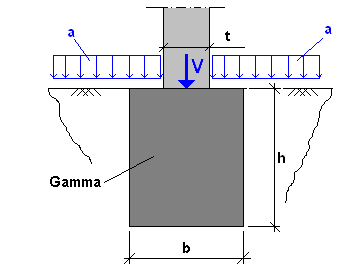
\includegraphics[scale=2]{Streifenfundament.png}
\caption{Schnitt durch ein Streifenfundament \cite{streifenfundament}}
\end{figure}
Es wird ein Streifenfundament gewählt, da hier besonders die räumliche Enge in Verbund mit großen Lasten ein Einzelfundament unwirtschaftlich macht. Es wird bewehrt ausgeführt um Rissbildung zu reduzieren. 
\subsubsection{Zugfundament}
\subsubsection*{Pfahlgründung}
Pfähle tragen Lasten über Mantelreibung und Spitzenwiderstand ab. Da bei einem Zugfundament kein Spitzenwiderstand wirkt, kann hier nur die Mantelreibung wirken. Unter Umständen werden deshalb sehr lange Pfähle benötigt, was in diesem Fall problematisch sein kann, da ab 5m Tiefe leicht betonagressives Grundwasser ansteht.
\subsubsection*{Streifenfundament}
Im Gegensatz zum Druckfundament wirkt das Streifenfundament bei Zugbelastung nur über Das Eigengewicht. Durch die Ausbildung als Streifenfundament können trotz geringer Tiefe und Breite durch die große Länge sehr schnell große Gewichte erzeugt werden.
\subsubsection*{Gewählte Variante: Streifenfundament}
Auch bei der Wahl für das Zugfundament spielten geometrische Faktoren eine Rolle. Da durch das agressive Grundwasser eine maximale Länge für Pfähle gesetzt ist, wird hier ein Streifenfundament gewählt. Außerdem hat dies technologische Vorteile, da beide Fundamente als Streifenfundament ausgeführt werden und so einige Arbeitsschritte kombiniert werden können.
\subsection{Berechnung des Druckfundamentes}
Berechnung nach \cite[S.107ff]{wsp}.
\subsubsection{Eingangswerte}
Das Fundament wird mittig mit einer vertikalen Last von 4300kN ständig und 550kN veränderlich pro Binder belastet. Der Binderabstand beträgt 9m. Für frostfreie Grüdung wird mindestens 1m tief gegründet.
\subsubsection*{Berechnung der Windlast}
Berechnung nach \cite[3.25]{schneider}.\\
Annahme: Windzone 1, Gebäudehöhe $10m < h \le 18m$ $\rightarrow$ $q_P = 0.65kN/m^2$\\
Der Wind wirkt pro Träger auf eine Fläche von 9mx13m (BinderabstandxHöhe).\\
Horizontallast pro Stütze: $0.65*9*13 = 76.05kN$


\subsubsection{Bestimmung der geometrischen Abmessungen}
\subsubsection*{Abschätzung der Fundamentfläche}
\begin{equation*}
A \approx \frac{V}{\frac{\sigma_{R.d}}{1.4}-\sigma_g}
\end{equation*}
\begin{itemize}
\item[] V = charakteristische äußere Last = 4850kN
\item[] $\sigma_{g} \approx \sqrt{V}/3$ bewehrter Beton $= 23.21kN/m^2$
\item[] \cite[S.111]{wsp}: Geschätzte Breite 2m, $\sigma_{R,d} = 430kN/m^2$, weder Abminderung noch Erhöhung, inkl. Begrenzung der Setzungen
\item[] $A \approx \frac{4850}{\frac{430}{1.4}-23.21} = 17.08m^2$
\end{itemize}
\subsubsection*{Festlegung der Abmessungen}
Erforderlich ist eine Fundamentfläche von $17m^2$ pro Binder. Bei einem Binderabstand von 9m werden 2m Fundamentbreite gewählt $(\widehat{=}18m^2) $
\subsubsection{Berechnung der Schnittgrößen}
\begin{itemize}
\item[] $V_k = 4850kN$
\item[] $G_k = 1m*2m*23*9mkN/m^3 = 414kN$
\item[] $H_k = 76.05kN$
\item[] $N_k = V_k + G_k = 5264kN$
\item[] $M_k = H_k * h = 76.05*1m = 76.05kNm$
\item[] $e = M_k/N_k = 76.05/5264 = 0.014m$
\item[] $\tan\delta_E = H_k/V_k = 76.05/5264 = 0.014 < 0.2$ notwenig für vereinfachten Nachweis.
\end{itemize}
Um den vereinfachten Nachweis anwenden zu können müssen die zulässige Ausmitte und der Nachweis gegen Kippen eingehalten werden.
\subsubsection{Nachweis Kippsicherheit GZ EQU}
Nach \cite[S.97]{wsp}\\
Da e sehr klein ist, wird direkt geprüft ist, ob die Ausmitte aus ständigen und veränderlichen Belastungen in der ersten Kernweite liegt. Damit wären beide Nachweise direkt erfüllt (größere Last oder kleinere zulässige Ausmitte).
\begin{itemize}
\item[] $e \le b/6 = 2m/6 = 0.33m$
\item[] $e = 0.014m < 0.33m \checkmark$
\end{itemize}
\subsubsection{Vereinfachter Nachweis}
Berechnung der reduzierten Fundamentfläche nach \cite[S.108]{wsp}.
\begin{itemize}
\item[] $b_L = b - e = 2m-0.014m = 1.986m$
\item[] $\sigma_{E,d} \le \sigma_{R,d}$
\item[] $\sigma_{E,d} = V_d/A' = (1.35V_g + 1.5V_p) / 18m^2 = (1.35*4300 + 1.5*550)/(9*1.986) = 370.93kN/m^2$
\item[] $\sigma_{R,d} = 430kN/m^2$ (s.o.)
\item[] $\sigma_{E,d} = 370.93kN/m^2 < 430kN/m^2 = \sigma_{R,d}\checkmark$
\end{itemize}
\subsection{Berechnung des Zugfundamentes}
Bei der Berechnung des Zugfundamentes wird die Reibung vernachlässigt und die Last alleine über das Gewicht abgetragen. Für frostfreie Gründung wird mindestens 1m tief gegründet.
\begin{itemize}
\item[] Nachweis: $Z_d <  G_d$
\item[] $Z_d = \gamma_G*Z_g + \gamma_Q*G_p = 1.35*1100 + 1.5*250 = 1860kN$
\item[] $G_d = G_k/\gamma_R = G_k/1.4$
\item[] erforderliches $G_k = 1860kN*1.4 = 2604kN$
\item[] Wichte des Stahlbetons $\gamma = 23kN/m^3$
\item[] Erforderliches Volumen: $V_min = 2604/23 = 113.23m^3$
\item[] Wirkende Länge des Fundamentes: $9m$
\item[] Nötige Querschnittsfläche: $A_{min} = 113.23/9 = 12.58m^2$
\item[] Gewählte Fläche: Breite $3.5m$, Tiefe $4m$, Fläche $14m^2$
\end{itemize}
\subsubsection{Verformung am Zugfundament infolge der Bauabschnitte}
Die Größte Verformung findet statt, wenn das Fundament schon gegossen wurde, aber die Halle noch nicht montiert ist. Zu berechnen sind also Setzungen aus Eigengewicht für das Zugfundament. Da keine horizontale Last angreift, sind nur mittlere Setzungen, also Setzungen aus zentrischer Last zu berechnen. Nach \cite[S.68]{wsp}.
\begin{itemize}
\item[] $s_m = \sigma_1bf/E_m$
\item[] $\sigma_1 = \sigma_0 = V/(9*3.5) = 9*4*3.5*23/(9*3.5) = 92kN/m^2$
\item[] $b = 3.5m$
\item[] $E_m = E_S/\kappa = 50/(2/3) = 75000kN/m^2$, $\kappa = 2/3$ für Sand und Schluff
\item[] $a/b = 9/4 = 2.25$
\item[] $f = 1.244$
\item[] $s_m = 92*3.5*1.244/75000 = 5.34mm$
\end{itemize}
Die Setzungen sind gering auch während des Bauzustandes \cite[S.37]{wsp} und beeinflussen deshalb nicht die Lösung.

\newpage
\section{Abbildungsverzeichnis}
\listoffigures
\newpage
\section{Literatur}
\begin{thebibliography}{9}
\bibitem[Spundwandhandbuch]{spund} 
http://www.thyssenkrupp-bautechnik.de/fileadmin/Leistungen/01 \_Spundwandprofile/\_media/spundwandhandbuch.pdf
\bibitem[Wikipedia - Gabione]{gabio} http://upload.wikimedia.org/wikipedia/de/3/3b/Gabionenwand.png
\bibitem[Schneider]{gewichtsmauer} Schneider Bautabellen, 20. Auflage
\bibitem[Seib Natursteine GmbH]{gabio2} http://www.seib-natursteine.com/gfx\_content/produktbilder/14030100.jpg
\bibitem[WSP]{wsp} Wissensspeicher Geotechnik - Delef Rütz, Karl Josef Witt - 18.Auflage - Weimar 2011
\bibitem[Paul Debus]{me} Paul Debus - Powered by Faber Castell
\bibitem[Schneider]{schneider} Schneider Bautabellen - 19. Auflage
\bibitem[Harzer-Statik-Software]{streifenfundament} http://www.harzerstatik.de/images/Programme/Grundbau/Streifenfundament/Systemgrafik-1-Streifenfundament.png
\end{thebibliography}

\end{document}
